% questions.tex —— 2010 年·普通高等学校招生考试·辽宁卷·理科 · 题目内容片段（无答案）
% 由 tools/generate_projects.py 依来源总账自 2010/2010_数学真题_辽宁理_试题.md 生成，勿手改（改源 MD 后重跑）
状态：needs-review；依固定候选 PDF 两页（印刷页 611–612）逐题核验，五幅图已矢量重绘。原页未印分值，不补。
原页第 22–24 题连续排在第 21 题之后，未另立「选考题」栏目名；按课标卷体例，这三题属选修模块选考（几何证明选讲、坐标系与参数方程、不等式选讲），三选一。
\gkpart{一、选择题}
\begin{question}
\gkti{1}已知 $A$，$B$ 均为集合 $U=\{1,3,5,7,9\}$ 的子集，且 $A\cap B=\{3\}$，$\complement_U B\cap A=\{9\}$，则 $A=$（　）

（A）$\{1,3\}$

（B）$\{3,7,9\}$

（C）$\{3,5,9\}$

（D）$\{3,9\}$

\end{question}
\begin{question}
\gkti{2}设 $a$，$b$ 为实数，若复数 $\dfrac{1+2\mathrm i}{a+b\mathrm i}=1+\mathrm i$，则（　）

（A）$a=\dfrac32$，$b=\dfrac12$

（B）$a=3$，$b=1$

（C）$a=\dfrac12$，$b=\dfrac32$

（D）$a=1$，$b=3$

\end{question}
\begin{question}
\gkti{3}两个实习生每人加工一个零件，加工为一等品的概率分别为 $\dfrac23$ 和 $\dfrac34$，两个零件是否加工为一等品相互独立，则这两个零件中恰有一个一等品的概率为（　）

（A）$\dfrac12$

（B）$\dfrac{5}{12}$

（C）$\dfrac14$

（D）$\dfrac16$

\Needspace{0.4\textheight}
\end{question}
\begingroup
\renewenvironment{question}{\Needspace{0.5\textheight}}{}
\begin{question}
\gkti{4}如果执行如图所示的程序框图，输入正整数 $n$，$m$，满足 $n\geqslant m$，那么输出的 $p$ 等于（　）

（A）$\mathrm C_n^{m-1}$

（B）$\mathrm A_n^{m-1}$

（C）$\mathrm C_n^{m}$

（D）$\mathrm A_n^{m}$
\nopagebreak[4]
\begin{center}% 2010 年辽宁卷理科第 4 题：程序框图。
% 来源 PDF：普通高考/2010/2010辽宁理.pdf，SHA-256 ba46f70f9d718652c24d14b28a0b473b768e864248ff0a9f1feb2374aec708f9。
% 原页：第 1 页（A3 三栏）第 1 栏中部，书页码 611。
% 重绘依据：照原页竖排主干 开始→输入 n,m→k=1,p=1→p=p(n-m+k)→判断 k<m?
%   「是」向右再向上进入右侧 k=k+1 框，该框顶部再向左汇入 p=p(n-m+k) 上方主干（循环体为
%   p=p(n-m+k)、k=k+1）；「否」向下经「输出 p」到「结束」。
\begin{tikzpicture}[semithick,
  every node/.style={inner sep=2pt},
  box/.style={draw, minimum width=3.7cm, minimum height=0.62cm, align=center},
  round/.style={draw, rounded corners=6pt, minimum width=1.7cm,
    minimum height=0.62cm, align=center},
  para/.style={draw, trapezium, trapezium left angle=70, trapezium right angle=110,
    minimum width=2.5cm, minimum height=0.66cm, align=center},
  dec/.style={draw, diamond, aspect=2.2, minimum width=2.6cm,
    minimum height=1.05cm, align=center},
  arr/.style={->, >=stealth}]

  \node[round] (start) at (0,0) {开始};
  \node[para]  (in)    at (0,-1.15) {输入 $n,\,m$};
  \node[box]   (init)  at (0,-2.32) {$k=1$，$p=1$};
  \node[box]   (prod)  at (0,-3.62) {$p=p(n-m+k)$};
  \node[box]   (inc)   at (4.15,-3.62) {$k=k+1$};
  \node[dec]   (test)  at (0,-5.05) {$k<m$};
  \node[para]  (out)   at (0,-6.40) {输出 $p$};
  \node[round] (end)   at (0,-7.50) {结束};

  \draw[arr] (start) -- (in);
  \draw[arr] (in) -- (init);
  \draw[arr] (init) -- (prod);
  \draw[arr] (test) -- (out);
  \node[right] at (0.18,-5.85) {否};
  \draw[arr] (out) -- (end);

  % 「是」分支：由判断框右侧向右、再向上进入 k=k+1
  \draw[arr] (test.east) -| (inc.south);
  \node[above] at (1.65,-5.03) {是};

  % 回边：k=k+1 顶部向上、再向左汇入 p=p(n-m+k) 上方主干
  \draw (inc.north) -- (4.15,-2.95) -- (0,-2.95);
\end{tikzpicture}
\end{center}
\nopagebreak[4]
\end{question}
\endgroup
\begin{question}
\gkti{5}设 $\omega>0$，函数 $y=\sin\left(\omega x+\dfrac{\pi}{3}\right)+2$ 的图象向右平移 $\dfrac{4\pi}{3}$ 个单位后与原图象重合，则 $\omega$ 的最小值是（　）

（A）$\dfrac23$

（B）$\dfrac43$

（C）$\dfrac32$

（D）$3$

\end{question}
\begin{question}
\gkti{6}设 $\{a_n\}$ 是由正数组成的等比数列，$S_n$ 为其前 $n$ 项和。已知 $a_2a_4=1$，$S_3=7$，则 $S_5=$（　）

（A）$\dfrac{15}{2}$

（B）$\dfrac{31}{4}$

（C）$\dfrac{33}{4}$

（D）$\dfrac{17}{2}$

\end{question}
\begin{question}
\gkti{7}设抛物线 $y^2=8x$ 的焦点为 $F$，准线为 $l$，$P$ 为抛物线上一点，$PA\perp l$，$A$ 为垂足，如果直线 $AF$ 的斜率为 $-\sqrt3$，那么 $|PF|=$（　）

（A）$4\sqrt3$

（B）$8$

（C）$8\sqrt3$

（D）$16$

\end{question}
\begin{question}
\gkti{8}平面上 $O$，$A$，$B$ 三点不共线，设 $\overrightarrow{OA}=\boldsymbol a$，$\overrightarrow{OB}=\boldsymbol b$，则 $\triangle OAB$ 的面积等于（　）

（A）$\sqrt{|\boldsymbol a|^2|\boldsymbol b|^2-(\boldsymbol a\cdot\boldsymbol b)^2}$

（B）$\sqrt{|\boldsymbol a|^2|\boldsymbol b|^2+(\boldsymbol a\cdot\boldsymbol b)^2}$

（C）$\dfrac12\sqrt{|\boldsymbol a|^2|\boldsymbol b|^2-(\boldsymbol a\cdot\boldsymbol b)^2}$

（D）$\dfrac12\sqrt{|\boldsymbol a|^2|\boldsymbol b|^2+(\boldsymbol a\cdot\boldsymbol b)^2}$

\end{question}
\begin{question}
\gkti{9}设双曲线的一个焦点为 $F$，虚轴的一个端点为 $B$，如果直线 $FB$ 与该双曲线的一条渐近线垂直，那么此双曲线的离心率为（　）

（A）$\sqrt2$

（B）$\sqrt3$

（C）$\dfrac{\sqrt3+1}{2}$

（D）$\dfrac{\sqrt5+1}{2}$

\end{question}
\begin{question}
\gkti{10}已知点 $P$ 在曲线 $y=\dfrac{4}{\mathrm e^x+1}$ 上，$\alpha$ 为曲线在点 $P$ 处的切线的倾斜角，则 $\alpha$ 的取值范围是（　）

（A）$\left[0,\dfrac{\pi}{4}\right)$

（B）$\left[\dfrac{\pi}{4},\dfrac{\pi}{2}\right)$

（C）$\left(\dfrac{\pi}{2},\dfrac{3\pi}{4}\right]$

（D）$\left[\dfrac{3\pi}{4},\pi\right)$

\end{question}
\begin{question}
\gkti{11}已知 $a>0$，则 $x_0$ 满足关于 $x$ 的方程 $ax=b$ 的充要条件是（　）

（A）$\exists x\in\mathbf R$，$\dfrac12ax^2-bx\geqslant\dfrac12ax_0^2-bx_0$

（B）$\exists x\in\mathbf R$，$\dfrac12ax^2-bx\leqslant\dfrac12ax_0^2-bx_0$

（C）$\forall x\in\mathbf R$，$\dfrac12ax^2-bx\geqslant\dfrac12ax_0^2-bx_0$

（D）$\forall x\in\mathbf R$，$\dfrac12ax^2-bx\leqslant\dfrac12ax_0^2-bx_0$

\end{question}
\begin{question}
\gkti{12}有四根长都为 $2$ 的直铁条，若再选两根长都为 $a$ 的直铁条，使这六根铁条端点处相连能够焊接成一个三棱锥形的铁架，则 $a$ 的取值范围是（　）

（A）$(0,\sqrt6+\sqrt2)$

（B）$(1,2\sqrt2)$

（C）$(\sqrt6-\sqrt2,\sqrt6+\sqrt2)$

（D）$(0,2\sqrt2)$

\end{question}
\gkpart{二、填空题}
\begin{question}
\gkti{13}$(1+x+x^2)\left(x-\dfrac1x\right)^6$ 的展开式中的常数项为 $\underline{\qquad}$。

\end{question}
\begin{question}
\gkti{14}已知 $-1<x+y<4$ 且 $2<x-y<3$，则 $z=2x-3y$ 的取值范围是 $\underline{\qquad}$。（答案用区间表示）

\Needspace{0.4\textheight}
\end{question}
\begingroup
\renewenvironment{question}{\Needspace{0.5\textheight}}{}
\begin{question}
\gkti{15}如图，网格纸的小正方形的边长是 $1$，在其上用粗线画出了某多面体的三视图，则这个多面体最长的一条棱的长为 $\underline{\qquad}$。
\nopagebreak[4]
\begin{center}% 2010 年辽宁卷理科第 15 题：网格纸上的三视图（正视图、侧视图、俯视图）。
% 来源 PDF：普通高考/2010/2010辽宁理.pdf，SHA-256 ba46f70f9d718652c24d14b28a0b473b768e864248ff0a9f1feb2374aec708f9。
% 原页：第 1 页（A3 三栏）第 2 栏下部，书页码 611。
% 重绘依据：照原页 L 形网格——上块 8 列 × 4 行，左下块另起 4 列 × 3 行，共 7 行；
%   左上是正视图（直角边在右、下，斜边自左下至右上），右上是侧视图（直角边在左、下，
%   斜边自左上至右下），左下是俯视图（正方形加一条自左下至右上的对角线）。
%   网格用细灰线，三视图轮廓用粗黑线。
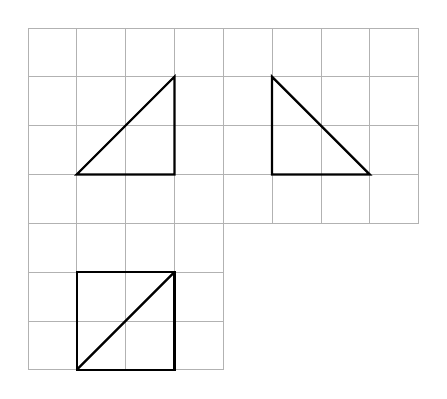
\begin{tikzpicture}[scale=0.62]
  % 网格：上块 8×4（y=3..7 满宽），左下块 4×3（y=0..3 仅左 4 列）
  \foreach \y in {0,1,2} {
    \draw[gray!60, very thin] (0,\y) -- (4,\y);
  }
  \foreach \y in {3,4,5,6,7} {
    \draw[gray!60, very thin] (0,\y) -- (8,\y);
  }
  \foreach \x in {0,1,2,3,4} {
    \draw[gray!60, very thin] (\x,0) -- (\x,7);
  }
  \foreach \x in {5,6,7,8} {
    \draw[gray!60, very thin] (\x,3) -- (\x,7);
  }

  % 正视图（左上）：直角边 2、2，斜边自左下至右上
  \draw[thick] (1,4) -- (3,4) -- (3,6) -- cycle;
  % 侧视图（右上）：直角边 2、2，斜边自左上至右下
  \draw[thick] (5,4) -- (7,4) -- (5,6) -- cycle;
  % 俯视图（左下）：正方形加一条对角线
  \draw[thick] (1,0) rectangle (3,2);
  \draw[thick] (1,0) -- (3,2);
\end{tikzpicture}
\end{center}
\nopagebreak[4]
\end{question}
\endgroup
\begin{question}
\gkti{16}已知数列 $\{a_n\}$ 满足 $a_1=33$，$a_{n+1}-a_n=2n$，则 $\dfrac{a_n}{n}$ 的最小值为 $\underline{\qquad}$。

\end{question}
\gkpart{三、解答题}
\begin{question}
\gkti{17}在 $\triangle ABC$ 中，$a$，$b$，$c$ 分别为内角 $A$，$B$，$C$ 的对边，且 $2a\sin A=(2b+c)\sin B+(2c+b)\sin C$。

（1）求 $A$ 的大小；

（2）求 $\sin B+\sin C$ 的最大值。

\Needspace{0.4\textheight}
\end{question}
\begingroup
\renewenvironment{question}{\Needspace{0.5\textheight}}{}
\begin{question}
\gkti{18}为了比较注射 $A$，$B$ 两种药物后产生的皮肤疱疹的面积，选 $200$ 只家兔做试验，将这 $200$ 只家兔随机地分成两组，每组 $100$ 只，其中一组注射药物 $A$，另一组注射药物 $B$。

（1）甲、乙是 $200$ 只家兔中的 $2$ 只，求甲、乙分在不同组的概率；

（2）下表 1 和表 2 分别是注射药物 $A$ 和 $B$ 后的试验结果。（疱疹面积单位：$\mathrm{mm}^2$）

表 1：注射药物 $A$ 后皮肤疱疹面积的频数分布表

\begin{center}
\begin{tabular}{lrrrr}
\toprule
疱疹面积 & $[60,65)$ & $[65,70)$ & $[70,75)$ & $[75,80)$ \\
\midrule
频数 & $30$ & $40$ & $20$ & $10$ \\
\bottomrule
\end{tabular}
\end{center}

表 2：注射药物 $B$ 后皮肤疱疹面积的频数分布表

\begin{center}
\begin{tabular}{lrrrrr}
\toprule
疱疹面积 & $[60,65)$ & $[65,70)$ & $[70,75)$ & $[75,80)$ & $[80,85)$ \\
\midrule
频数 & $10$ & $25$ & $20$ & $30$ & $15$ \\
\bottomrule
\end{tabular}
\end{center}

① 完成下面频率分布直方图，并比较注射两种药物后疱疹面积的中位数大小；
\nopagebreak[4]
\begin{center}% 2010 年辽宁卷理科第 18 题（2）①：两张待完成的频率分布直方图坐标系。
% 来源 PDF：普通高考/2010/2010辽宁理.pdf，SHA-256 ba46f70f9d718652c24d14b28a0b473b768e864248ff0a9f1feb2374aec708f9。
% 原页：第 1 页（A3 三栏）第 3 栏下部，书页码 611。
% 重绘依据：照原页画空坐标系（原页即要求学生补画小矩形）——纵轴「频率/组距」自
%   0.01 到 0.08，横轴 60 到 85（每 5 一格），纵横虚线网格、两轴各有一处断裂记号；
%   左为图 1：注射药物 A，右为图 2：注射药物 B。不代画柱形，保持与原页一致。
\begin{tikzpicture}[x=0.7cm, y=0.49cm, semithick]
  % ---------- 图 1：注射药物 A ----------
  \begin{scope}
    % 坐标轴
    \draw[->, >=stealth] (0,0) -- (0,9.15);
    \draw[->, >=stealth] (0,0) -- (7.05,0);
    % 虚线网格：竖线 x=1..6（即 60..85），横线 y=1..8（即 0.01..0.08）
    \foreach \i in {1,2,3,4,5,6} {
      \draw[dashed, dash pattern=on 3pt off 3pt] (\i,0) -- (\i,8);
    }
    \foreach \j in {1,2,3,4,5,6,7,8} {
      \draw[dashed, dash pattern=on 3pt off 3pt] (0,\j) -- (6,\j);
    }
    % 纵轴刻度值
    \foreach \j/\v in {1/0.01, 2/0.02, 3/0.03, 4/0.04, 5/0.05, 6/0.06, 7/0.07, 8/0.08} {
      \node[anchor=east, inner sep=1pt] at (-0.12,\j) {\v};
    }
    % 横轴刻度值
    \node[anchor=north, inner sep=2pt] at (0,-0.12) {0};
    \foreach \i/\v in {1/60, 2/65, 3/70, 4/75, 5/80, 6/85} {
      \node[anchor=north, inner sep=2pt] at (\i,-0.12) {\v};
    }
    % 轴断裂记号
    \draw (0.42,0.10) -- (0.56,-0.10) -- (0.70,0.10);
    \draw (0.62,0.10) -- (0.76,-0.10) -- (0.90,0.10);
    \draw (0.10,0.42) -- (-0.10,0.56) -- (0.10,0.70);
    % 轴名
    \node[align=center, inner sep=1pt] at (0.92,10.75) {频率};
    \draw[semithick] (0.36,10.25) -- (1.48,10.25);
    \node[align=center, inner sep=1pt] at (0.92,9.75) {组距};
    \node[anchor=west, inner sep=2pt] at (7.15,1.0) {疱疹面积};
    % 图题
    \node[anchor=north, inner sep=3pt] at (3,-1.05) {图 1：注射药物 $A$};
  \end{scope}

  % ---------- 图 2：注射药物 B ----------
  \begin{scope}[xshift=7.95cm]
    \draw[->, >=stealth] (0,0) -- (0,9.15);
    \draw[->, >=stealth] (0,0) -- (7.05,0);
    \foreach \i in {1,2,3,4,5,6} {
      \draw[dashed, dash pattern=on 3pt off 3pt] (\i,0) -- (\i,8);
    }
    \foreach \j in {1,2,3,4,5,6,7,8} {
      \draw[dashed, dash pattern=on 3pt off 3pt] (0,\j) -- (6,\j);
    }
    \foreach \j/\v in {1/0.01, 2/0.02, 3/0.03, 4/0.04, 5/0.05, 6/0.06, 7/0.07, 8/0.08} {
      \node[anchor=east, inner sep=1pt] at (-0.12,\j) {\v};
    }
    \node[anchor=north, inner sep=2pt] at (0,-0.12) {0};
    \foreach \i/\v in {1/60, 2/65, 3/70, 4/75, 5/80, 6/85} {
      \node[anchor=north, inner sep=2pt] at (\i,-0.12) {\v};
    }
    \draw (0.42,0.10) -- (0.56,-0.10) -- (0.70,0.10);
    \draw (0.62,0.10) -- (0.76,-0.10) -- (0.90,0.10);
    \draw (0.10,0.42) -- (-0.10,0.56) -- (0.10,0.70);
    \node[align=center, inner sep=1pt] at (0.92,10.75) {频率};
    \draw[semithick] (0.36,10.25) -- (1.48,10.25);
    \node[align=center, inner sep=1pt] at (0.92,9.75) {组距};
    \node[anchor=west, inner sep=2pt] at (7.15,1.0) {疱疹面积};
    \node[anchor=north, inner sep=3pt] at (3,-1.05) {图 2：注射药物 $B$};
  \end{scope}
\end{tikzpicture}
\end{center}
\nopagebreak[4]
② 完成下面 $2\times2$ 列联表，并回答能否有 $99.9\%$ 的把握认为“注射药物 $A$ 后的疱疹面积与注射药物 $B$ 后的疱疹面积有差异”。

\begin{center}
\begin{tabular}{lllr}
\toprule
 & 疱疹面积小于 $70\ \mathrm{mm}^2$ & 疱疹面积不小于 $70\ \mathrm{mm}^2$ & 合计 \\
\midrule
注射药物 $A$ & $a=$ & $b=$ &  \\
注射药物 $B$ & $c=$ & $d=$ &  \\
合计 &  &  & $n=$ \\
\bottomrule
\end{tabular}
\end{center}

\Needspace{5\baselineskip}
附：
\nopagebreak[4]
\[K^2=\frac{n(ad-bc)^2}{(a+b)(c+d)(a+c)(b+d)}.\]

\begin{center}
\begin{tabular}{lrrrrr}
\toprule
$P(K^2\geqslant k)$ & $0.100$ & $0.050$ & $0.025$ & $0.010$ & $0.001$ \\
\midrule
$k$ & $2.706$ & $3.841$ & $5.024$ & $6.635$ & $10.828$ \\
\bottomrule
\end{tabular}
\end{center}

\Needspace{0.4\textheight}
\end{question}
\endgroup
\begingroup
\renewenvironment{question}{\Needspace{0.5\textheight}}{}
\begin{question}
\gkti{19}已知三棱锥 $P-ABC$ 中，$PA\perp$ 平面 $ABC$，$AB\perp AC$，$PA=AC=\dfrac12AB$，$N$ 为 $AB$ 上一点，$AB=4AN$，$M$，$S$ 分别为 $PB$，$BC$ 的中点。

（1）证明：$CM\perp SN$；

（2）求 $SN$ 与平面 $CMN$ 所成角的大小。
\nopagebreak[4]
\begin{center}% 2010 年辽宁卷理科第 19 题：三棱锥 P-ABC 及点 M、S、N。
% 来源 PDF：普通高考/2010/2010辽宁理.pdf，SHA-256 ba46f70f9d718652c24d14b28a0b473b768e864248ff0a9f1feb2374aec708f9。
% 原页：第 2 页（A3 三栏）第 1 栏上部，书页码 612。
% 重绘依据：照原页——P 在最高处，B 在左下，C 在右且与 A 近乎等高，A 在形内偏左，
%   PA 为几乎竖直的虚线；M 在棱 PB 上，S 在棱 BC 上，N 在棱 AB 上（N 距 A 为 AB/4）。
%   可见棱 PB、PC、BC 与线段 MC 用实线；被遮挡的 PA、AB、AC 及辅助线 MN、CN、SN 用虚线。
\begin{tikzpicture}[scale=0.72, semithick, line join=round]
  \coordinate (B) at (0,0);
  \coordinate (A) at (2.6,3.2);
  \coordinate (C) at (7.4,3.2);
  \coordinate (P) at (3.0,7.4);
  \coordinate (M) at ($(P)!0.5!(B)$);
  \coordinate (S) at ($(B)!0.5!(C)$);
  \coordinate (N) at ($(A)!0.25!(B)$);

  % 可见棱：实线
  \draw (P) -- (B);
  \draw (P) -- (C);
  \draw (B) -- (C);
  % 线段 MC：实线（自 M 过 A 上方到 C）
  \draw (M) -- (C);

  % 被遮挡的棱与辅助线：虚线
  \draw[dashed] (P) -- (A);
  \draw[dashed] (A) -- (B);
  \draw[dashed] (A) -- (C);
  \draw[dashed] (M) -- (N);
  \draw[dashed] (N) -- (C);
  \draw[dashed] (N) -- (S);

  % M、S、N 处的等分记号（短横线）
  \draw ($(M)!0.07cm!90:(P)$) -- ($(M)!-0.07cm!90:(P)$);
  \draw ($(S)!0.07cm!90:(B)$) -- ($(S)!-0.07cm!90:(B)$);
  \draw ($(N)!0.07cm!90:(A)$) -- ($(N)!-0.07cm!90:(A)$);

  % 顶点标注
  \node[above] at (P) {$P$};
  \node[left]  at (B) {$B$};
  \node[right] at (C) {$C$};
  \node[above left, inner sep=1pt] at (A) {$A$};
  \node[left=3pt, inner sep=1pt] at (M) {$M$};
  \node[below left=1pt and 3pt, inner sep=1pt] at (N) {$N$};
  \node[below right, inner sep=1pt] at (S) {$S$};
\end{tikzpicture}
\end{center}
\nopagebreak[4]
\end{question}
\endgroup
\begin{question}
\gkti{20}设椭圆 $C:\dfrac{x^2}{a^2}+\dfrac{y^2}{b^2}=1$（$a>b>0$）的左焦点为 $F$，过点 $F$ 的直线与椭圆 $C$ 相交于 $A$，$B$ 两点，直线 $l$ 的倾斜角为 $60^\circ$，$\overrightarrow{AF}=2\overrightarrow{FB}$。

（1）求椭圆 $C$ 的离心率；

（2）如果 $|AB|=\dfrac{15}{4}$，求椭圆 $C$ 的方程。

\end{question}
\begin{question}
\gkti{21}已知函数 $f(x)=(a+1)\ln x+ax^2+1$。

（1）讨论函数 $f(x)$ 的单调性；

（2）设 $a<-1$，如果对任意 $x_1$，$x_2\in(0,+\infty)$，$|f(x_1)-f(x_2)|\geqslant4|x_1-x_2|$，求 $a$ 的取值范围。

\Needspace{0.4\textheight}
\end{question}
\begingroup
\renewenvironment{question}{\Needspace{0.5\textheight}}{}
\begin{question}
\gkti{22}如图，$\triangle ABC$ 的角平分线 $AD$ 的延长线交它的外接圆于点 $E$。

（1）证明：$\triangle ABE\sim\triangle ADC$；

（2）若 $\triangle ABC$ 的面积 $S=\dfrac12AD\cdot AE$，求 $\angle BAC$ 的大小。
\nopagebreak[4]
\begin{center}% 2010 年辽宁卷理科第 22 题：△ABC 的外接圆，角平分线 AD 的延长线交圆于 E。
% 来源 PDF：普通高考/2010/2010辽宁理.pdf，SHA-256 ba46f70f9d718652c24d14b28a0b473b768e864248ff0a9f1feb2374aec708f9。
% 原页：第 2 页（A3 三栏）第 2 栏下部，书页码 612。
% 重绘依据：照原页——BC 为水平弦（本图中恰为直径），A 在圆上偏左上方，E 在圆上偏下方；
%   AD 与 AE 是同一条直线，D 为它与 BC 的交点；线段 AB、AC、BC、AE、BE 均为实线。
\begin{tikzpicture}[scale=1.15, semithick, line join=round]
  \coordinate (O) at (0,0);
  \coordinate (B) at (180:2);
  \coordinate (C) at (0:2);
  \coordinate (A) at (123:2);
  \coordinate (E) at (266:2);
  \coordinate (D) at (intersection of A--E and B--C);

  \draw (O) circle[radius=2];

  \draw (A) -- (B);
  \draw (A) -- (C);
  \draw (B) -- (C);
  \draw (A) -- (E);
  \draw (B) -- (E);

  \node[above, inner sep=2pt] at (A) {$A$};
  \node[left, inner sep=2pt] at (B) {$B$};
  \node[right, inner sep=2pt] at (C) {$C$};
  \node[below right=1pt and 1pt, inner sep=1pt] at (D) {$D$};
  \node[below, inner sep=2pt] at (E) {$E$};
\end{tikzpicture}
\end{center}
\nopagebreak[4]
\end{question}
\endgroup
\begin{question}
\gkti{23}已知 $P$ 为半圆 $C:\begin{cases}x=\cos\theta,\\y=\sin\theta,\end{cases}$（$\theta$ 为参数，$0\leqslant\theta\leqslant\pi$）上的点，点 $A$ 的坐标为 $(1,0)$，$O$ 为坐标原点，点 $M$ 在射线 $OP$ 上，线段 $OM$ 与 $C$ 的弧 $\overset{\frown}{AP}$ 的长度均为 $\dfrac{\pi}{3}$。

（1）以 $O$ 为极点，$x$ 轴的正半轴为极轴建立极坐标系，求点 $M$ 的极坐标；

（2）求直线 $AM$ 的参数方程。

\end{question}
\begin{question}
\gkti{24}已知 $a$，$b$，$c$ 均为正数，证明：$a^2+b^2+c^2+\left(\dfrac1a+\dfrac1b+\dfrac1c\right)^2\geqslant6\sqrt3$，并确定 $a$，$b$，$c$ 为何值时，等号成立。

\end{question}